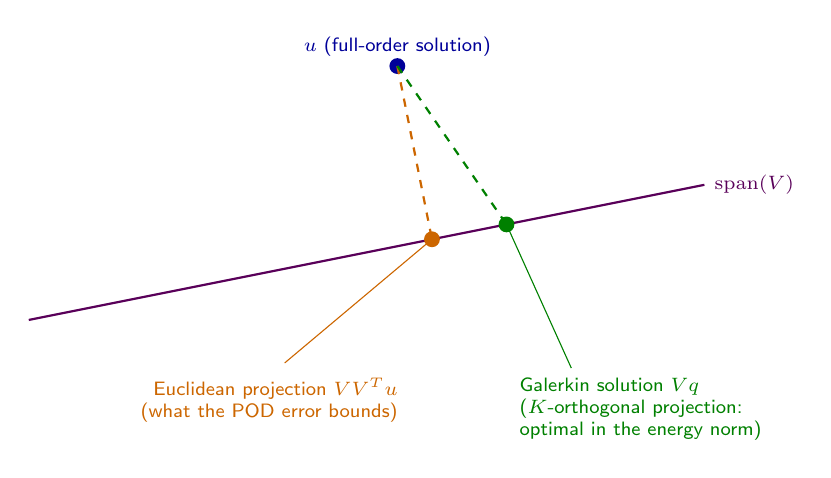
\begin{tikzpicture}[font=\sffamily\scriptsize,scale=1.3]
\draw[thick,violet!70!black] (-0.4,-0.08) -- (6.2,1.24) node[right] {$\mathrm{span}(\bm V)$};
\coordinate (U) at (3.2,2.4);
\coordinate (E) at (3.538,0.708);
\coordinate (G) at (4.266,0.853);
\fill[blue!60!black] (U) circle (2.2pt) node[above] {$\bm u$ (full-order solution)};
\fill[orange!80!black] (E) circle (2.2pt);
\fill[green!50!black] (G) circle (2.2pt);
\draw[dashed,orange!80!black,thick] (U) -- (E);
\draw[dashed,green!50!black,thick] (U) -- (G);
\node[orange!80!black,align=right,anchor=north east,font=\sffamily\scriptsize] at (3.3,-0.55) {Euclidean projection $\bm V\bm V^T\bm u$\\(what the POD error bounds)};
\draw[orange!80!black,->] (2.1,-0.5) -- (E);
\node[green!50!black,align=left,anchor=north west,font=\sffamily\scriptsize] at (4.3,-0.55) {Galerkin solution $\bm V\bm q$\\($\bm K$-orthogonal projection:\\optimal in the energy norm)};
\draw[green!50!black,->] (4.9,-0.55) -- (G);
\end{tikzpicture}
